\def\difficulty{1}
\sujet{Image Characterization}

\begin{note}This tutorial aims to characterize objects by geometrical and morphometrical measurements.
\end{note}

\index{Characterization}

\noindent The different processes will be applied on synthetic images as well as images from the Kimia database \cite{KimiaDB,Sharvit1998}:
{
\makeatletter
\renewcommand\fs@ruled{\def\@fs@cfont{\bfseries}\let\@fs@capt\floatc@ruled
	\def\@fs@pre{\hrule height.8pt depth0pt \kern2pt}%
	\def\@fs@post{\kern2pt\hrule\relax}%
	\def\@fs@mid{\vskip2pt}%
	\let\@fs@iftopcapt\iftrue}
\makeatother
\begin{figure}[H]
\centering
\subfloat[Bat.]{
\includegraphics[height=.3\linewidth]{bat-5.png}}\hfill
\subfloat[Camel.]{
\includegraphics[height=.3\linewidth]{camel-5.png}}\hfill
\subfloat[Ray.]{
\includegraphics[height=.3\linewidth]{ray-5.png}}
\vspace*{-9pt}
\end{figure}
}

\section{Perimeters}
\index{Characterization!Perimeter}
We are going to calculate the perimeter using the Crofton formula. This formula consists in integrating the intercept number of the object with lines of various orientation and positions.
Its expression in the 2-D planar case is given by:
$$
P(X)=\pi\int\chi(X\cap L)dL
$$
where the Euler-poincar\'e characteristic $\chi$ is equal to the number of connected components of the intersection of $X$ with a line $L$.\\
In the discrete case, the Crofton formula can be estimated by considering the intercept numbers for the horizontal $i_0$, vertical $i_{\pi/2}$ and diagonal orientations $i_{\pi/4}$ and $i_{3\pi/4}$ as:
$$
P(X)=\pi\times \frac{1}{4}\left(i_0+\frac{1}{\sqrt{2}}i_{\pi/4}+i_{\pi/2}+\frac{1}{\sqrt{2}}i_{3\pi/4}\right)
$$
\begin{qbox}
\begin{enumerate}
	\item Calculate the intercept number of a binary object from the Kimia database with lines oriented in the following four  directions: $0, \pi/4, \pi/2, 3\pi/4$.
	\item Deduce the value of the Crofton perimeter.
	\item Compare the result with the classical perimeter functions.
\end{enumerate}	
\end{qbox}

\begin{mcomment}
\begin{mremark}
See \minline{bwperim}.
\end{mremark}
\end{mcomment}

\begin{pcomment}
\begin{premark}
See \pinline{perimeter} from \pinline{skimage.measure}.
\end{premark}
\end{pcomment}


\section{Feret Diameter}\vspace*{-8pt}
 \index{Characterization!Diameter}
The Feret diameter (a.k.a. the caliper diameter) is the length of the projection of an object in one specified direction Fig.\ref{tut:image_characterization:enonce:feret_diameter}.

\vspace*{-10pt}

\begin{figure}[H]
 \centering\caption{Feret diameter of the object in horizontal direction.}%
 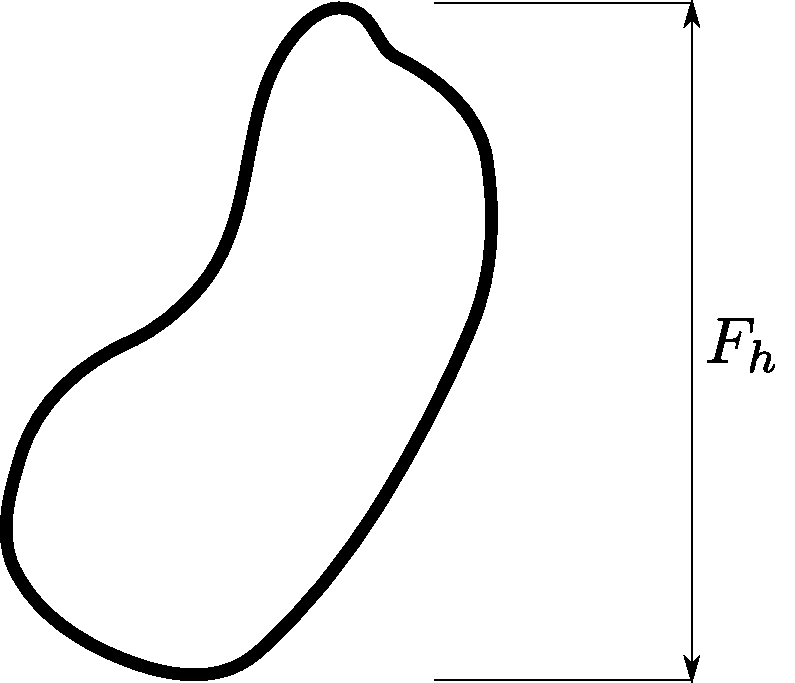
\includegraphics[width=4cm]{feret_diameter.pdf}%
 \label{tut:image_characterization:enonce:feret_diameter}%
\end{figure}

\vspace*{-10pt}

\begin{qbox}
\begin{enumerate}
	\item Calculate the projections in different directions of a binary object from the Kimia database.
	\item Deduce the minimum, maximum and mean value of the Feret diameters.
\end{enumerate}
\end{qbox}

\vspace*{-8pt}

\section{Circularity}\vspace*{-8pt}
\index{Characterization!Circularity}
We want to know if the object $X$ is similar to a disk. For that, we define the following measurement (circularity criterion):\vspace*{-10pt}
\[
circ(X)=\frac{4\pi A(X)}{P(X)^2}
\vspace*{-8pt}\]
where $A(X)$ and $P(X)$ denote the area and perimeter of the object $X$.

\begin{qbox}
\begin{enumerate}
	\item Show that the circularity of a disc is equal to $1$.
	\item Generate an array representing an object as a discrete disc. 
	\item Calculate its circularity and comment the results.
\end{enumerate}
\end{qbox}

\vspace*{-4pt}

\begin{mcomment}
\begin{mremark}
Use \minline{meshgrid}.
\end{mremark}
\end{mcomment}

\begin{pcomment}
\begin{premark}
Use \pinline{numpy.meshgrid}.
\end{premark}
\end{pcomment}


\section{Convexity}\vspace*{-8pt}
\index{Characterization!Convexity}
\index{Computational Geometry!Convex Hull}
We want to know if the object $X$ is convex. For that, we define the following measurement:\vspace*{-8pt}
$$
conv(X)=\frac{A(X)}{A(CH(X))}
$$
where $CH(X)$ denotes the filled convex hull of the object $X$.

\begin{qbox}
\begin{enumerate}
	\item Compute the convex hull of a pattern from the Kimia database.
	\item Evaluate the area of the filled convex hull.
	\item Deduce the convexity of the pattern.
\end{enumerate}
\end{qbox}

\vspace*{-4pt}

\begin{mcomment}
\begin{mremark}
See \minline{convhull} and \minline{poly2mask}.
\end{mremark}
\end{mcomment}


\begin{pcomment}
\begin{premark}
See \pinline{ConvexHull} from \pinline{scipy.spatial}.
\end{premark}
\end{pcomment}

